\chapter{Aspectos conceituais}
\label{CAP2}

A seguir serão explicados os conceitos fundamentais que possibilitam a execução deste trabalho. 

% apresentar conceitos empregados e revisao da literatura (parte toerica do trab)

\section{O padrão OBD-II}

Criado na década de 1990 para gerar controle sobre as emissões de gás carbônico dos carros\textsuperscript{[5]}, hoje define um protocolo padronizado para comunicar parâmetros internos do veículo.
    
O padrão OBD-II foi uma extensão do padrão OBD-I, uniformizando esse tipo de conector em casos em geral, começando a ser adotado no Brasil a partir de 2010\textsuperscript{[4]}.

A comunicação é feita através de uma conexão física que normalmente pode ser encontrada abaixo do volante do motorista\textsuperscript{[5]}, conforme indicado pela figura \ref{fig:obd2_conn}.

Nesse padrão de conexão e comunicação é definida uma interface por onde parâmetros internos a um carro podem ser monitorados.

As mensagens definidas pelo OBD-II têm cada uma um PID (parameter ID). O conjunto comum de PIDs de serviços que podem ser solicitados pela porta OBD-II e para que servem pode ser visto na tabela \ref{Tb:tab1}\textsuperscript{[3]}.

\begin{table}[]
% \begin{adjustbox}{width=\textwidth}
\begin{tabular}{cc}
\rowcolor[HTML]{656565} 
{\color[HTML]{FFFFFF} Service / Mode (hex)} & {\color[HTML]{FFFFFF} Description}                                                                    \\
01                                          & Show current data - I/M Monitors and Live Data                                                        \\
02                                          & Show Freeze Frame (FF) Data                                                                           \\
03                                          & Show Stored Diagnostic Trouble Codes                                                                  \\
04                                          & Clear/Erase Diagnostic Trouble Codes and stored values                                                \\
05                                          & Test results, oxygen sensor monitoring (non CAN only)                                                 \\
06                                           & Test results, other component/system monitoring (Test results, oxygen sensor monitoring for CAN only) \\
07                                           & Show pending Diagnostic Trouble Codes (detected during current or last driving cycle)                 \\
08                                           & Control operation of on-board component/system (EVAP)                                                 \\
09                                          & Request Vehicle Information (VIN)                                                                     \\
0A                                          & Permanent Diagnostic Trouble Codes (DTCs) (Cleared DTCs)                                             
\end{tabular}
\end{table}

É importante notar que os serviços do padrão OBD-II comuns a todos os carros sempre começam com o dígito zero (hexadecimal), por isso, serviços específicos de cada fabricante devem começam a partir do código 0x10.

\begin{figure}[hp]
    \centering
    
    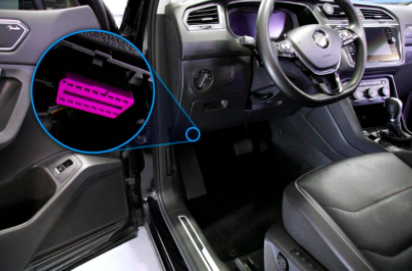
\includegraphics[]{figures/localizacao_obd2.png}
    
    \caption{Posição da porta OBD-II em um carro\textsuperscript{[5]}}
    
    \label{fig:obd2_conn}
\end{figure}

Os dados que podem ser coletados de qualquer carro são explicitados na tabela \ref{Tb:tab2}\textsuperscript{[3]}.

% Please add the following required packages to your document preamble:
% \usepackage[table,xcdraw]{xcolor}
% If you use beamer only pass "xcolor=table" option, i.e. \documentclass[xcolor=table]{beamer}
\begin{table}[]
\begin{tabular}{ccccccc}
\rowcolor[HTML]{C0C0C0} 
{\color[HTML]{FFFFFF} \textbf{PIDs(hex)}} & {\color[HTML]{FFFFFF} \textbf{PID(Dec)}} & {\color[HTML]{FFFFFF} \textbf{Data bytes returned}} & {\color[HTML]{FFFFFF} \textbf{Description}} & {\color[HTML]{FFFFFF} \textbf{Min value}} & {\color[HTML]{FFFFFF} \textbf{Max value}} & {\color[HTML]{FFFFFF} \textbf{Units}} \\
04                                         & 4                                        & 1                                                   & Calculated engine load                      & 0                                         & 100                                       & \%                                    \\
0C                                        & 12                                       & 2                                                   & Engine speed                                & 0                                         & 16,383.75                                 & rpm                                   \\
0D                                        & 13                                       & 1                                                   & Vehicle speed                               & 0                                         & 255                                       & km/h                                  \\
0F                                        & 15                                       & 1                                                   & Intake air temperature                      & -40                                       & 215                                       & °C                                    \\
1F                                        & 31                                       & 2                                                   & Run time since engine start                 & 0                                         & 65,535                                    & seconds                               \\
33                                        & 51                                       & 1                                                   & Absolute Barometric Pressure                & 0                                         & 255                                       & kPa                                   \\
46                                        & 70                                       & 1                                                   & Ambient air temperature                     & -40                                       & 215                                       & °C                                    \\
47                                        & 71                                       & 1                                                   & Absolute throttle position B                & 0                                         & 100                                       & \%                                    \\
49                                        & 73                                       & 1                                                   & Accelerator pedal position D                & 0                                         & 100                                       & \%                                    \\
51                                        & 81                                       & 1                                                   & Fuel Type                                   & -                                         & -                                         & -                                     \\
52                                        & 82                                       & 1                                                   & Ethanol fuel \%                             & 0                                         & 100                                       & \%                                    \\
5A                                        & 90                                       & 1                                                   & Relative accelerator pedal position         & 0                                         & 100                                       & \%                                    \\
5B                                        & 91                                       & 1                                                   & Hybrid battery pack remaining life          & 0                                         & 100                                       & \%                                    \\
5C                                        & 92                                       & 1                                                   & Engine oil temperature                      & -40                                       & 210                                       & °C                                    \\
5D                                        & 93                                       & 2                                                   & Fuel injection timing                       & -210.00                                   & 301992                                    & °                                     \\
5E                                        & 94                                       & 2                                                   & Engine fuel rate                            & 0                                         & 3212.75                                   & L/h                                   \\
61                                        & 97                                       & 1                                                   & Driver's demand engine - percent torque     & -125                                      & 130                                       & \%                                    \\
62                                        & 98                                       & 1                                                   & Actual engine - percent torque              & -125                                      & 130                                       & \%                                    \\
63                                        & 99                                       & 2                                                   & Engine reference torque                     & 0                                         & 65,535                                    & Nm                                    \\
64                                        & 100                                      & 5                                                   & Engine percent torque data                  & -125                                      & 130                                       & \%                                    \\
70                                        & 112                                      & 10                                                  & Boost pressure control                      & -                                         & -                                         & -                                     \\
83                                        & 131                                      & 9                                                   & NOx sensor                                  & -                                         & -                                         & -                                     \\
8E                                        & 142                                      & 1                                                   & Engine Friction - Percent Torque            & -125                                      & 130                                       & \%                                   
\end{tabular}
\end{table}

Interessante notar que, embora não esteja representado na tabela, os PIDs 0x00, 0x20, 0x40, etc, ou seja, a cada 32 valores de PID, existe um parâmetro apenas para indicar quais entre os PIDs seguintes são fornecidos por aquele carro.

Esses PIDs de marcação, por assim dizer, utilizam 4 bytes para comunicar quais dos próximos PIDs estão disponíveis, utilizando cada bit como uma flag binária. 

Na figura \ref{fig:bitwise_obd2} é possível visualizar como esse processo é feito, usando como exemplo o valor 0xBE1FA813 para representar os 4 bytes oferecidos\textsuperscript{[3]}.

\begin{figure}[hp]
    \centering
    
    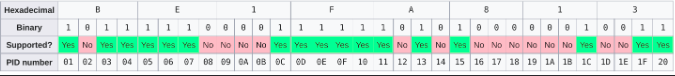
\includegraphics[scale=0.7]{figures/tabela_dados_disponiveis.png}
    
    \caption{Divisão bit a bit da mensagem OBD-II informando os serviços disponíveis\textsuperscript{[3]}}
    
    \label{fig:bitwise_obd2}
\end{figure}

A coleta de fato dos dados relevantes será feita por uma aplicação desenvolvida \textit{a priori} que já é capaz de comunicar-se corretamente com a interface OBD.

Essa aplicação acelerará a criação da infraestrutura proposta por este trabalho, uma vez que pula o primeiro passo da estratégia \textit{bottom-up} que deverá permear o projeto.

\section{Transmissão de dados}

A implementação da transmissão \textit{Bluetooth} neste projeto de compilação de dados oferece uma solução eficaz para a comunicação entre os produtor e consumidor de dados. 

Ao utilizar essa tecnologia, os dados de rastreamento podem ser transmitidos de forma sem fio e em tempo real para dispositivos equipados com \textit{Bluetooth}, como \textit{smartphones}, que são o foco deste trabalho.

A abordagem \textit{wireless} proporciona uma conectividade mais flexível, eliminando a necessidade de cabos físicos e simplificando a integração do sistema. A baixa energia do \textit{Bluetooth} permite uma transmissão eficiente de dados, minimizando o impacto no consumo de bateria dos dispositivos móveis.

Além disso, a transmissão \textit{Bluetooth} possibilita a interação direta entre o sistema de geração e os usuários, permitindo a visualização em tempo real de informações de condução.

Essa integração sem fio não apenas aprimora a experiência do usuário, mas também amplia as possibilidades de interatividade e controle, tornando o sistema mais acessível e fácil de usar.

 \begin{figure}[hp]
    \centering
    
    
\includegraphics[scale=0.4]{figures/bluetooth.png}
    
    \caption{Logo do Bluetooth.}
    
\end{figure}

\section{Armazenamento em nuvem}
Provedoras como a Amazon e a Azure (Microsoft) oferecem serviços de nuvem que podem ser usados para este projeto \textsuperscript{[10, 11]}. Neste trabalho, optou-se pelo serviço da AWS, uma vez que um dos integrantes do grupo já tinha familiaridade com o serviço.

A integração do aplicativo Android com o Amazon RDS (Relational Database Service) da AWS oferece uma solução eficiente e escalável para o armazenamento de dados. 

Utilizando o RDS, os dados coletados, como informações de localização, velocidade e aceleração, podem ser armazenados em bancos de dados relacionais, proporcionando alta disponibilidade, segurança e desempenho otimizado. 

A flexibilidade do Amazon RDS permite a escolha de diferentes motores de banco de dados, como MySQL, PostgreSQL, ou SQL Server, adequando-se às necessidades específicas do sistema.

Os usuários poderão transmitir informações para a nuvem a qualquer momento, desde que seus carros estejam ligados e conectados à internet. O volume de dados recebidos no sistema é, portanto, variável e por isso fez sentido que o serviço de nuvem contratado siga o modelo \textit{on demand}. A figura \ref{figure:custo_aws_inicial} mostra o custo calculado no serviço da AWS RDS.

\begin{figure}[hp]
    \centering
    
    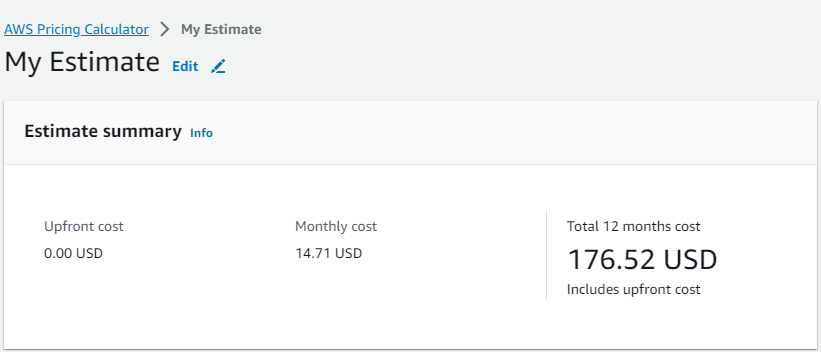
\includegraphics[scale=0.8]{figures/custo_aws_inicial.PNG}
    \caption{Custo da AWS.}
    \label{figure:custo_aws_inicial}
    
\end{figure}

A região do Leste da Virgina é conhecida por ter uma alta densidade de \textit{data centers}. Isso resulta em eficiência operacional e redução de custos.

A instância escolhida foi a \textbf{db.t3.micro}. Ela é uma instância de banco de dados pequena, sendo adequada para cargas de trabalho leves. Essa instância é comumente usada para ambientes de desenvolvimento, testes ou pequenas aplicações que não exigem muitos recursos.

Um RDS Proxy é um serviço que facilita a escalabilidade e a alta disponibilidade para as conexões de banco de dados. Ele ajuda a melhorar o desempenho e a segurança ao gerenciar as conexões entre seus aplicativos e instâncias de banco de dados RDS. Isso é especialmente útil em ambientes onde há flutuações na carga de trabalho. Como se trata de um protótipo, não há preocupações com carga de trabalho. Logo, essa opção não foi escolhida.

Também não há necessidade de ter um ambiente de zona de disponibilidade múltipla para garantir escalabilidade, pois haveria custo adicional. Por isso, a instância RDS foi configurada para o modo Single-AZ. E a capacidade de armazenamento foi 20 GB.

As figuras \ref{figure:custo_aws_configuracao_1}, \ref{figure:custo_aws_configuracao_2} e \ref{figure:custo_aws_configuracao_3} mostram a configuração no serviço da AWS RDS.

\begin{table}[]
\begin{tabular}{llllll}
\multicolumn{5}{c}{\textbf{Amazon RDS para MySQL}}                                                           &  \\
                                               &        &  &                  &                              &  \\
\textbf{Escolha o tipo de localização}         & Região &  & Escolha a região & \textbf{US East(N.Virginia)} &  \\
                                               &        &  &                  &                              &  \\
                                               &        &  &                  &                              &  \\
\textbf{Especificação das instancias do MySql} &        &  &                  &                              &  \\
\textbf{Quantidade}                            & 1      &  &                  &                              &  \\
                                               &        &  &                  &                              &  \\
\textbf{Instância Selecionada}                 &        &  &                  &                              &  \\
db.t3.micro                                    &        &  &                  &                              &  \\
vCPU:2                                         &        &  &                  &                              &  \\
Memória: 1 GiB                                 &        &  &                  &                              & 
\end{tabular}
\end{table}

 
\begin{figure}[hp]
    \centering
    
    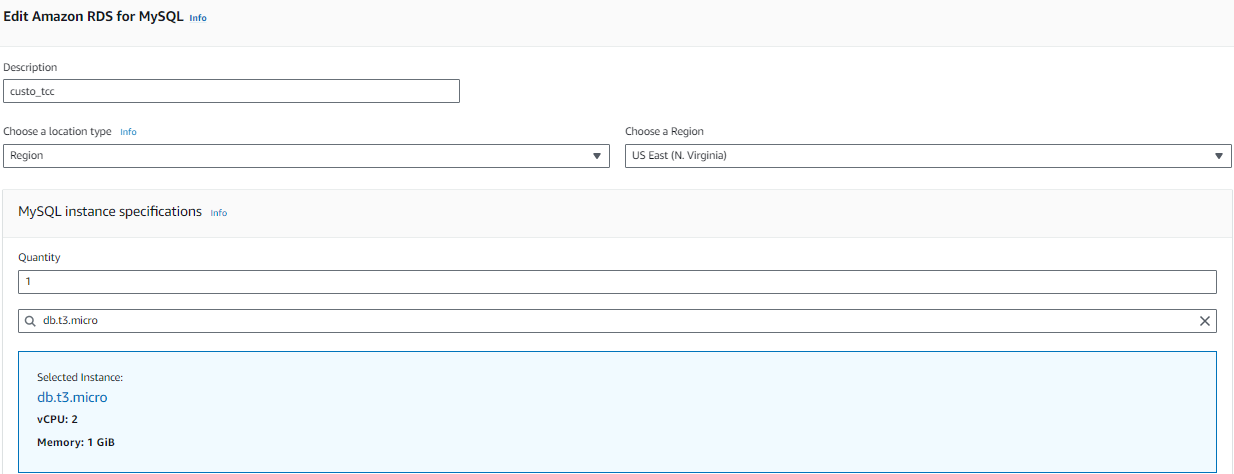
\includegraphics[scale=0.5]{figures/custo_aws_configuracao.PNG}
    \caption{Custo da AWS - Configuração 1.}
    \label{figure:custo_aws_configuracao_1}
    
\end{figure}

\begin{figure}[hp]
    \centering
    
    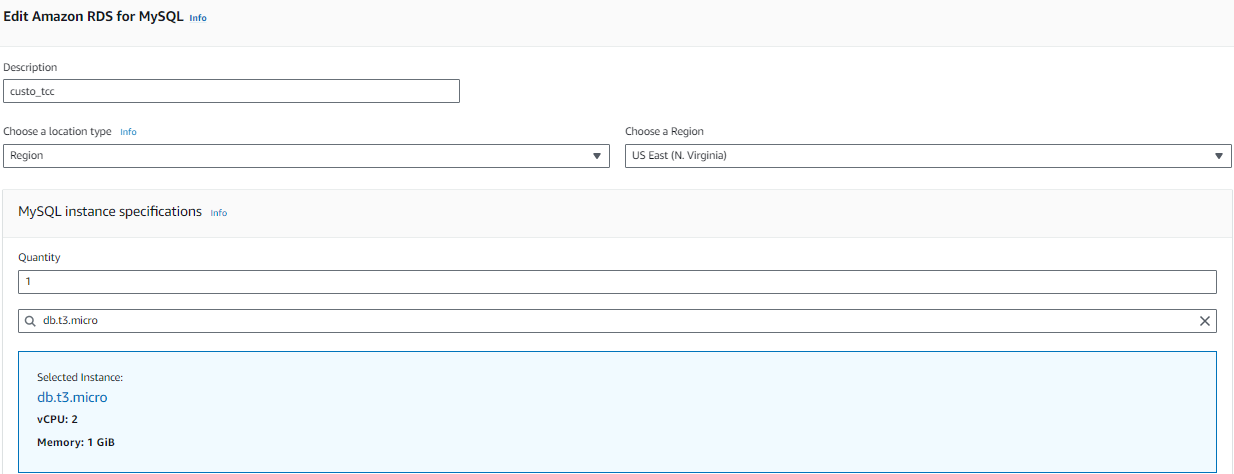
\includegraphics[scale=0.5]{figures/custo_aws_configuracao.PNG}
    \caption{Custo da AWS - Configuração 2.}
    \label{figure:custo_aws_configuracao_2}
    
\end{figure}

\begin{figure}[hp]
    \centering
    
    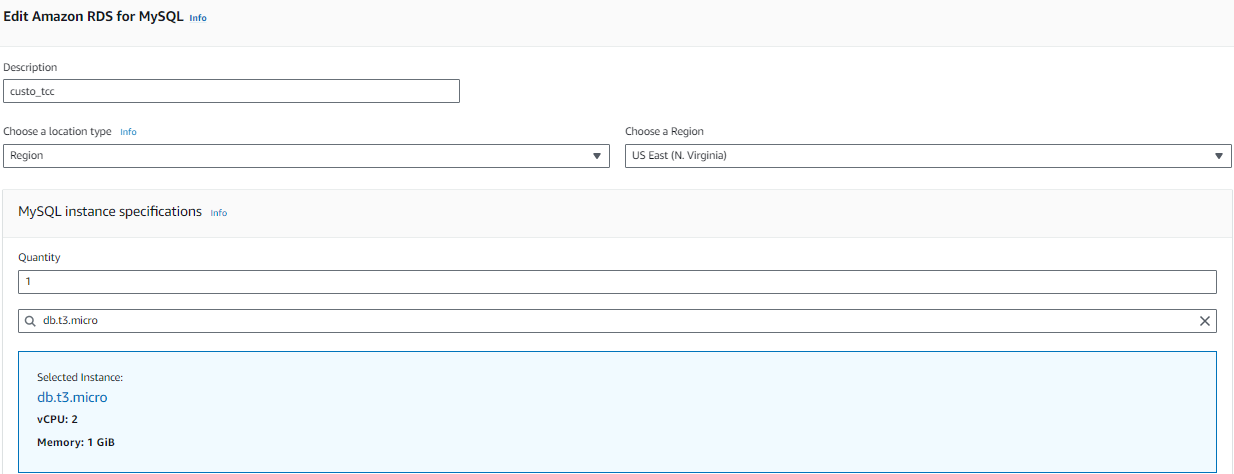
\includegraphics[scale=0.5]{figures/custo_aws_configuracao.PNG}
    \caption{Custo da AWS - Configuração 3.}
    \label{figure:custo_aws_configuracao_3}
    
\end{figure}